\section{Orbital Design}

\subsection{Semi Walker Delta Configuration}

In order to reduce the necessary costs to design this satellite-based constellation some other configurations will be discussed. The Walker Delta Configuration (WDC) represents the most general constellation for a given inclination different to 90 degrees, i.e. 75 degrees. The WDC is a uniform based 360 degree generated configuration with equidistant orbits, which implies a certain redundant Earth coverage as described in the previous chapter.However, this can and will be solved by generating a 180 degree constellation - Semi Walker Delta Configuration (SWDC) - which will also fulfill global coverage although having some inconvenients. 

\begin{figure}[h]
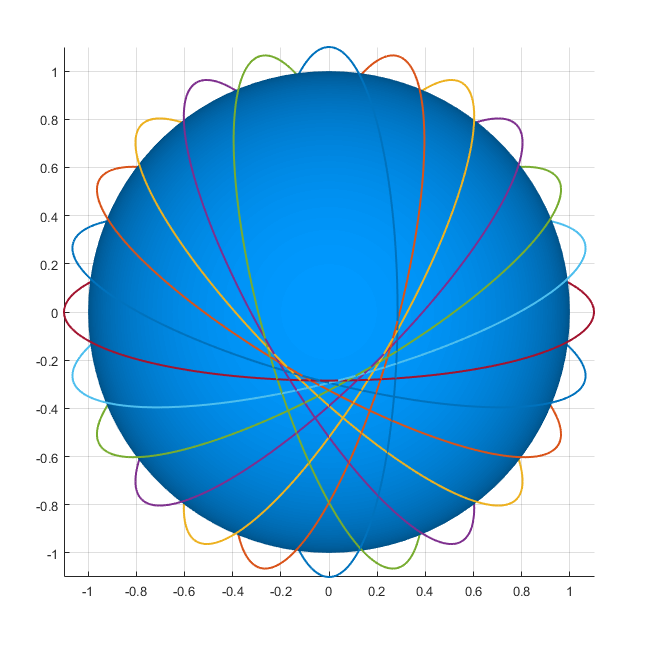
\includegraphics[width=12cm]{semiwalker12vertical}
\centering
\caption{12 plane SWDC. Note the gap and the equidistant planes}
\end{figure}

\subsubsection{Advantages}
-	\textbf{Distance between planes reduced.} With the SWDC constellation the redundant orbits are directly corrected, thus the distance between planes is reduced to half, as results from the geometry itself.

-	\textbf{Less number of planes needed.} This means that in order to approach global coverage fewer planes will be requiered due to the decrease in distance between planes.
 
-	\textbf{Satellites following the same direction - sense} With the SWDC constellation the orbits have no interaction with each other, thus the satellites for each orbit can be set following the same direction. This will significantly improve the communications among satellites from different planes; also, we will be avoiding the Doppler Effect.

\begin{figure}[h]
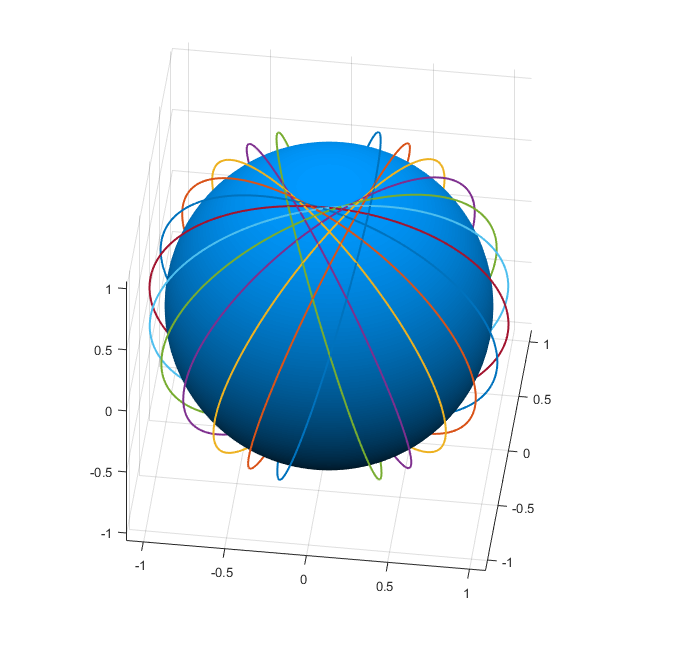
\includegraphics[width=12cm]{semiwalker12}
\centering
\caption{This geometry distribution induces a large anti-symmetric gap}
\end{figure}

\subsubsection{Disadvantages}
-	\textbf{Gap configuration.} With the SWDC constellation the main problem is the gap that results from configuring the constellation at a given inclination and describing equidistant orbits. In order to fulfull global coverage this gap will have to be covered by means of auxiliar orbits.

\subsection{Other Walker Delta Configurations}
As we have discussed for the SWDC, the main disadvantage respect to the Walker Delta Configuration is the fact that a gap is obtained, thus a global coverage network cannot be described. In order to cover the entire Earth we have analysed some ways of covering the gap with auxiliar orbits.

\subsubsection{SWDC including an additional polar orbit.}
This polar orbit would be set directly on top of the gap described by the SWDC. The main issue with polar orbits, as discussed before in this report, is the complex reorientation and decay in inclination that takes place. We must take into account these considerations when covering the entire Earth, especially if we only have one polar orbit in our constellation. 

\begin{figure}[h]
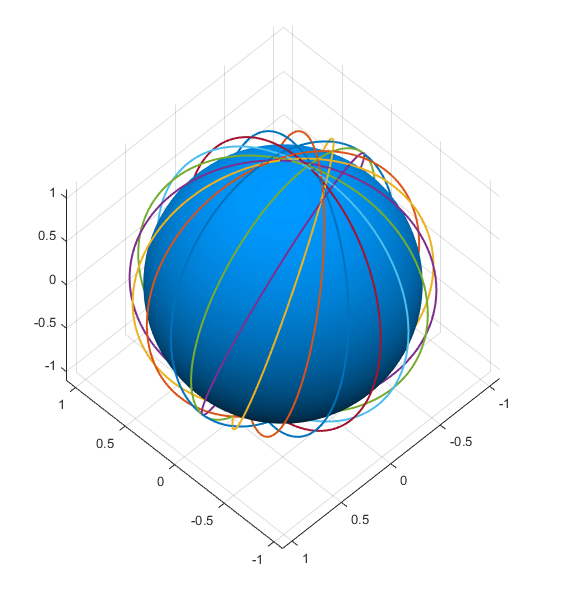
\includegraphics[width=10cm]{semiwalker11p1}
\centering
\caption{Added polar orbit to the 11 plane based SWDC}
\end{figure}

\subsubsection{Mixed Walker Delta.}
In order to avoid using polar orbits and their complex reorientations, we can contemplate adding planes to the SWDC. In result, different configurations distributed around the Earth can be described and set in order to fulfill global coverage. As discussed before, the SWDC constellation is generated around 180 degrees whereas the Walker Delta Constellation is a 360 degree generated configuration. This Mixed Walker Delta (MWDC) is the result of adding some planes to the SWDC, thus a constellation can be generated for different degree values, such as 210, 225, 240, etc. 

\begin{figure}[h]
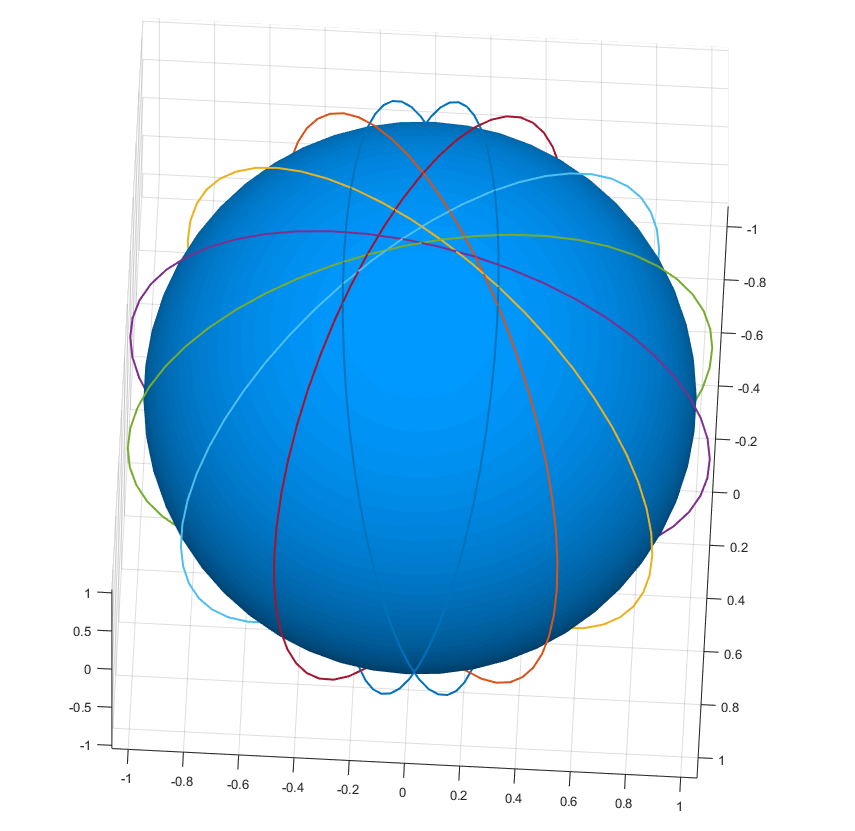
\includegraphics[width=10cm]{MWDC}
\centering
\caption{8 plane based MWDC generated for 210 degrees}
\end{figure}

After different mathematical approaches and optimal solutions, the department of Orbital Design considered that the best option in order to have a global coverage constellation with the least economic and strategic issues - exposed and discussed in previous chapters - would be that of a 210 degree generated MWDC, defined by 9 planes and 21 satellites per plane. This configuration was found optimizing the whole Earth in order to have full coverage without gaps (except for the limitations of this model at high latitudes). An important consideration is that we also analysed other Mixed Walker Delta Configurations for 210 and 240 degrees, but these resulted in a more expensive distribution of satellites.